\section{Unseen granularities and context response}
\label{app:scale-continuum}

\paragraph{Figure~\ref{fig:granularity-query-summary}: evaluation and aggregation.}
All three panels use eight sections excluded from pretraining, with the encoder and transformation frozen. In panels (a,b), target MSE compares unchanged source states and ZoomST predictions against the same directly encoded targets. Panel (a) averages the trained pairs $8\to32$, $8\to128$ and $32\to128$ within each section, using all section positions. Panel (b) averages the six unseen targets $12,16,24,48,64,96$ queried from $e_8$ at 1,024 fixed positions per section. Panel (c) selects the lowest and highest predicted-response quarters separately within each section and doubling interval ($8\to16$, $16\to32$, $32\to64$, $64\to128$), with 256 locations per quarter, then averages their directly encoded changes over the four intervals. Each box therefore contains eight section means. The highest-response quarter shows larger encoded changes than the lowest quarter in 31 of 32 section--interval conditions (Figure~\ref{fig:granularity-query-summary}c).

\subsection{Transition heads on a shared frozen encoder}
\label{app:transition-comparison}

\paragraph{Shared-encoder comparison.}
The neural ODE and granularity-conditioned residual MLP are trained at 8, 32 and 128 on a shared frozen encoder, then evaluated against the same directly encoded targets. Averaging MSE over six unseen granularities, the ODE reduces error on every held-out section, with a mean paired reduction of 10.86\% (Figure~\ref{fig:ode-transition-comparison}).

\begin{figure}[!htbp]
\centering
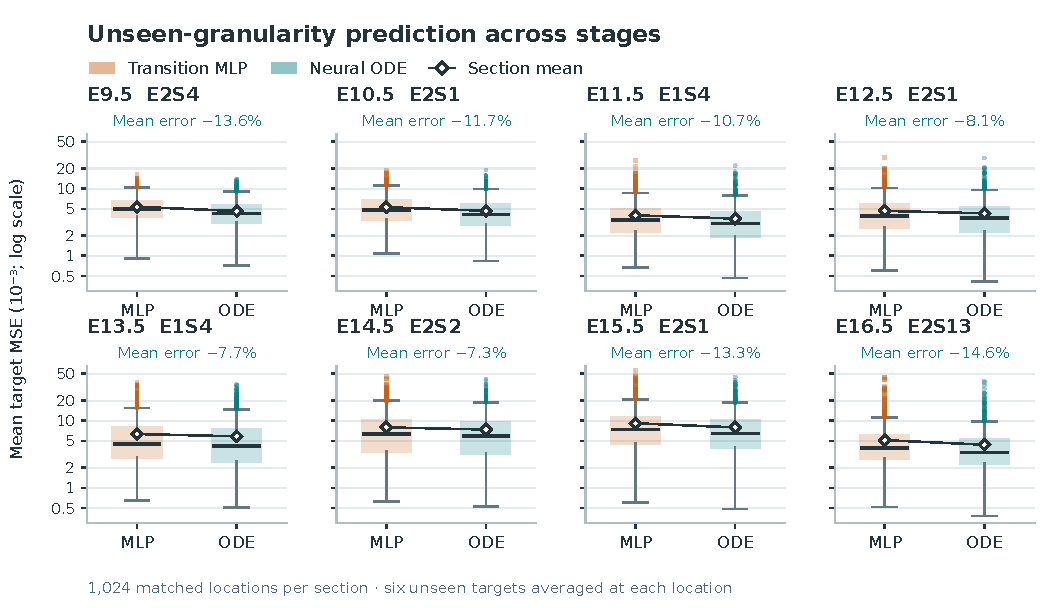
\includegraphics[width=\linewidth]{figures/ode_vs_transition_boxplots.pdf}
\caption{\textbf{Lower mean unseen-granularity error with neural ODE.} Each panel compares the granularity-conditioned residual MLP and ODE on one held-out section. Both heads use the same frozen encoder, fine-state inputs and directly encoded targets. Each box contains 1,024 location-level MSEs, each averaged equally over $k\in\{12,16,24,48,64,96\}$. Boxes show medians and interquartile ranges; whiskers extend to 1.5 interquartile ranges, with all outliers shown. Connected diamonds mark section means; percentages give their paired relative reductions. All panels share the same logarithmic axis.}
\label{fig:ode-transition-comparison}
\end{figure}

We compare the ODE with the granularity-conditioned residual MLP,
\[
T^{\mathrm{MLP}}_{a\to b}(z)=z+\mathrm{MLP}\!\left([\mathrm{LN}(z),h(a),h(b),u(b)-u(a)]\right).
\]
The MLP has dimensions $321\to128\to256$ with GELU activation and 32-dimensional scale embeddings; the ODE field has dimensions $257\to128\to256$. For a query between adjacent trained coordinates $u_j,u_{j+1}$, the MLP uses $h(k)=(1-w)h_j+wh_{j+1}$ with $w=(u(k)-u_j)/(u_{j+1}-u_j)$. The heads contain 74,848 and 66,560 trainable parameters, respectively.

Both heads are initialized afresh and trained on the same frozen encoder outputs from all 45 source sections for two epochs (7,224 updates; batch 1,024). AdamW uses learning rate $2\times10^{-4}$, 188 warmup steps and cosine decay to one tenth of the peak rate; gradient norms are clipped at five. Weight decay is 0.02 for weight matrices, 0.01 for scale embeddings and zero for normalization and bias terms. The ODE uses RK4 with maximum step 0.25 in $u$. Evaluation uses the same 1,024 positions per held-out section and the same directly encoded targets for both heads.

For section $s$, let $M_s^m$ be its MSE averaged equally over the six unseen targets for head $m$. The mean paired reduction is $100\,\mathrm{mean}_s(1-M_s^{\mathrm{ODE}}/M_s^{\mathrm{MLP}})=10.86\%$, ranging from 7.28\% to 14.56\% across sections. Table~\ref{tab:ode-transition-frozen} gives the section summaries underlying Figure~\ref{fig:ode-transition-comparison}. These are separately fitted transition heads on a common reference encoder.

\begin{table}[!htbp]
\centering\small
\caption{\textbf{Matched transition heads on a shared frozen encoder.} MSE is averaged over all six unseen targets and 1,024 locations per section. The mean reduction averages the eight paired section reductions.}
\label{tab:ode-transition-frozen}
\begin{tabular}{lccc}
\toprule
Section & MLP MSE ($\times10^{-3}$) & ODE MSE ($\times10^{-3}$) & Reduction (\%) \\
\midrule
E9.5 E2S4 & 5.381 & 4.650 & 13.57 \\
E10.5 E2S1 & 5.303 & 4.682 & 11.73 \\
E11.5 E1S4 & 4.014 & 3.585 & 10.69 \\
E12.5 E2S1 & 4.673 & 4.295 & 8.08 \\
E13.5 E1S4 & 6.342 & 5.853 & 7.71 \\
E14.5 E2S2 & 7.971 & 7.391 & 7.28 \\
E15.5 E2S1 & 9.174 & 7.957 & 13.26 \\
E16.5 E2S13 & 5.140 & 4.392 & 14.56 \\
Mean & 6.000 & 5.350 & 10.86 \\
\bottomrule
\end{tabular}

\end{table}

\subsection{Agreement with unseen neighborhood encodings}
\label{app:unseen-state-detail}

\paragraph{Frozen state prediction.}
The MOSTA encoder and ODE transition are frozen after joint training at 8,32,128. We use 1,024 fixed positions on each of the eight held-out sections and directly encode neighborhoods at $\mathcal K=\{8,12,16,24,32,48,64,96,128\}$. The molecular encoding procedure and neighborhood ordering remain unchanged. All predictions start from the same $e_{i,8}$; the encoded intermediate states are scoring references and do not enter these predictions.

Let $\widehat e_i(k)=T_{8\to k}(e_{i,8})$ and $\mathcal U=\mathcal K\setminus\{8,32,128\}$. For section $s$, target MSE averages $d^{-1}\|\widehat e_i(k)-e_i(k)\|^2$ over positions. The section's relative gain is one minus its MSE averaged over $k\in\mathcal U$ divided by the corresponding unchanged-$e_8$ MSE. Gains are then averaged over eight sections, yielding 21.96\%. Normalized RMSE divides RMSE by the target's root-mean-square variation around its section mean, so $R^2=1-\mathrm{NRMSE}^2$ within each section. Prediction improves over unchanged $e_8$ in all 48 section--target conditions. Figure~\ref{fig:granularity-query-summary}b plots absolute MSE averaged over the six targets within each section, giving eight paired section means.

\paragraph{Distance to a common directly encoded target.}
For the direct-distance comparison in Figure~\ref{fig:ode-unseen-distance-distributions}, define
\[
d_i^{\mathrm{start}}(k)=\frac{\|e_{i,8}-e_i(k)\|_2}{\sqrt d},\qquad
d_i^{\mathrm{pred}}(k)=\frac{\|\widehat e_i(k)-e_i(k)\|_2}{\sqrt d}.
\]
At each target, we average these per-position RMS distances within each section. Sections receive equal weight in the summary. Averaging $1-\overline d_s^{\mathrm{pred}}(k)/\overline d_s^{\mathrm{start}}(k)$ equally over the six unseen targets and eight sections gives a 10.38\% reduction, ranging from 3.04\% to 20.55\% across the 48 conditions. Every condition has a lower mean and median prediction distance. Within individual conditions, 81.15--99.71\% of positions are closer to the target. This RMS-distance statistic differs from the reduction in mean squared error reported above.

\begin{figure}[!htbp]
\centering
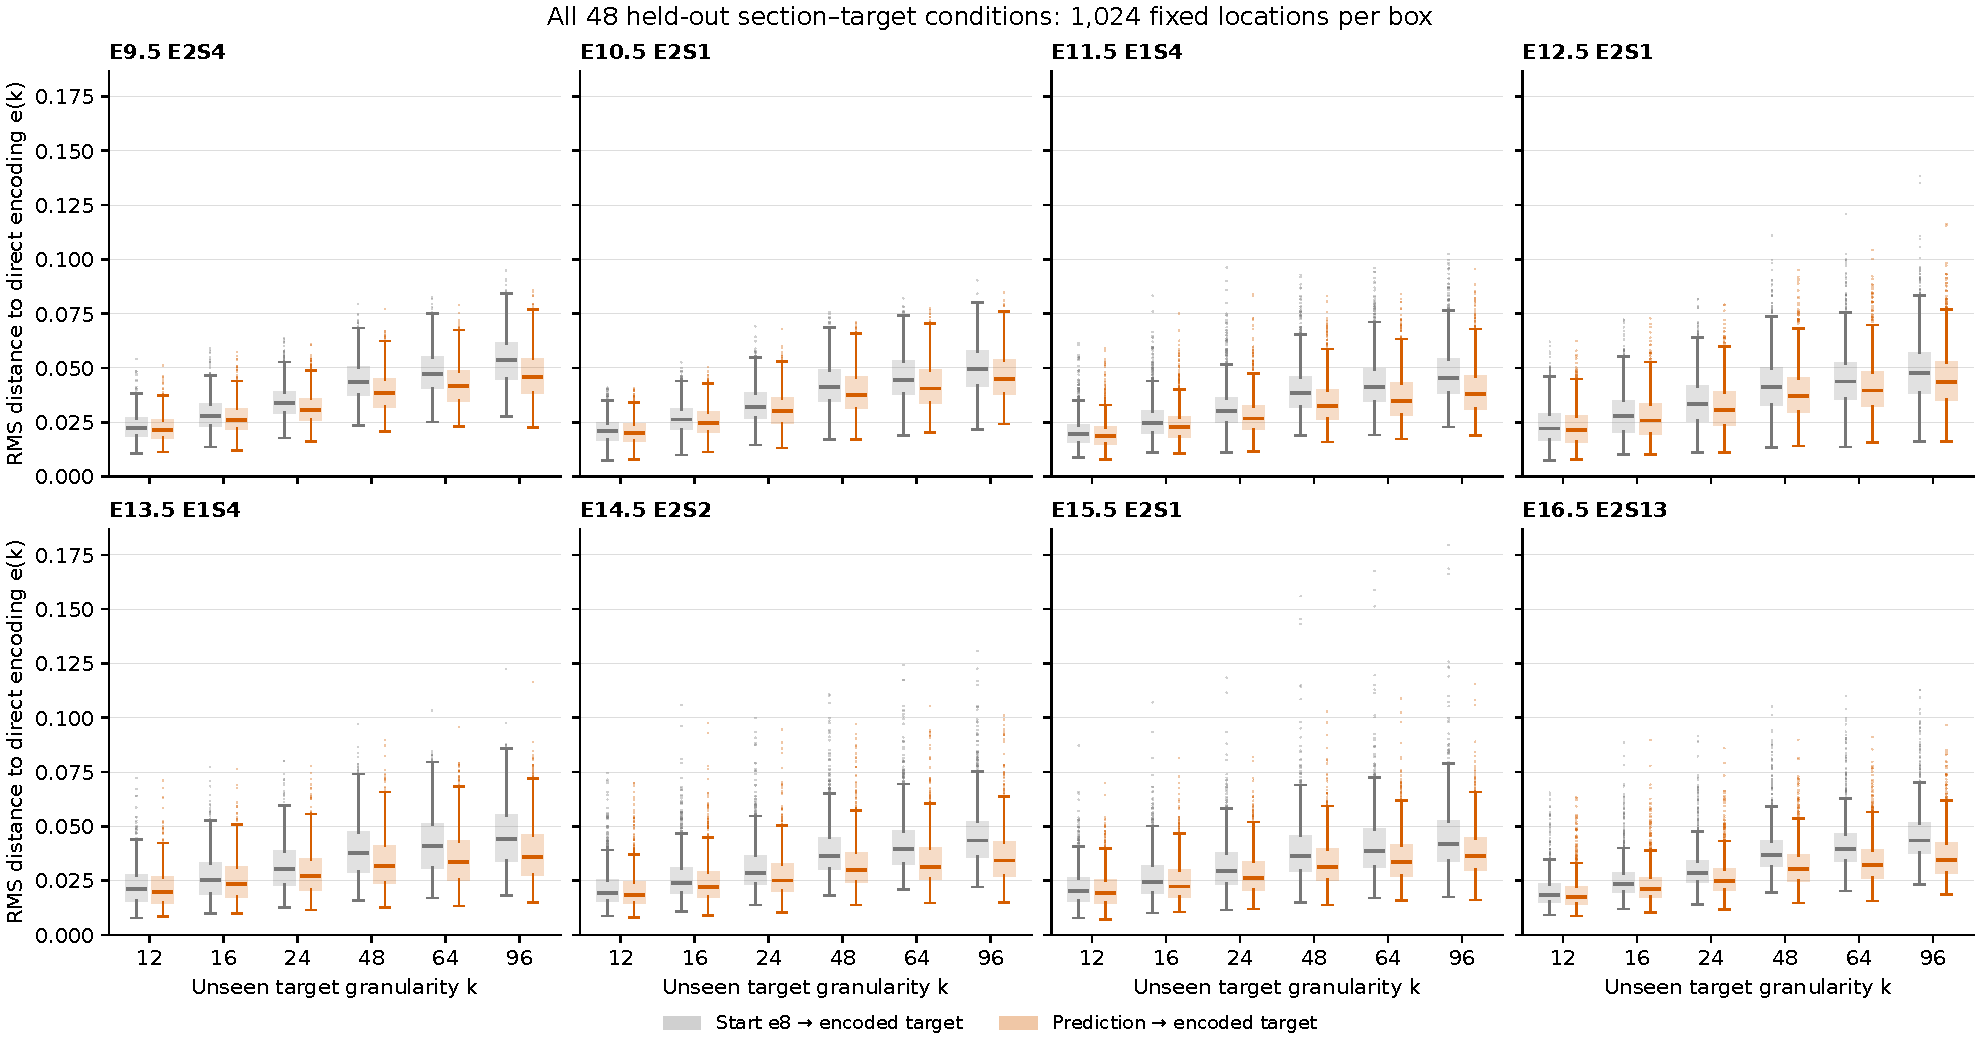
\includegraphics[width=\linewidth]{figures/unseen_state_distances_all_sections.pdf}
\caption{\textbf{Within-section distributions of distance to directly encoded unseen states.} The panels cover eight held-out sections and six unseen target granularities. Each pair compares distances from unchanged $e_8$ and from the prediction to the same target at the same 1,024 fixed positions. Boxes show medians and interquartile ranges, whiskers extend to 1.5 interquartile ranges, and outliers are retained. Position distributions describe each section; section means are the units in the main comparison.}
\label{fig:ode-unseen-distance-distributions}
\end{figure}

\paragraph{Shared-space visualization and full-state error.}
The E16.5 E1S1 analysis uses 1,024 fixed positions. We fit a center-only, full-SVD PCA on the directly encoded states at all nine granularities, then apply the same mean and components to predictions. All positions are shown with common axis limits. The first two PCs explain 20.25\% and 17.02\% of encoded-state variance. Table~\ref{tab:ode-case-pca} reports prediction accuracy in the full 256-dimensional space.

\begin{figure}[!htbp]
\centering
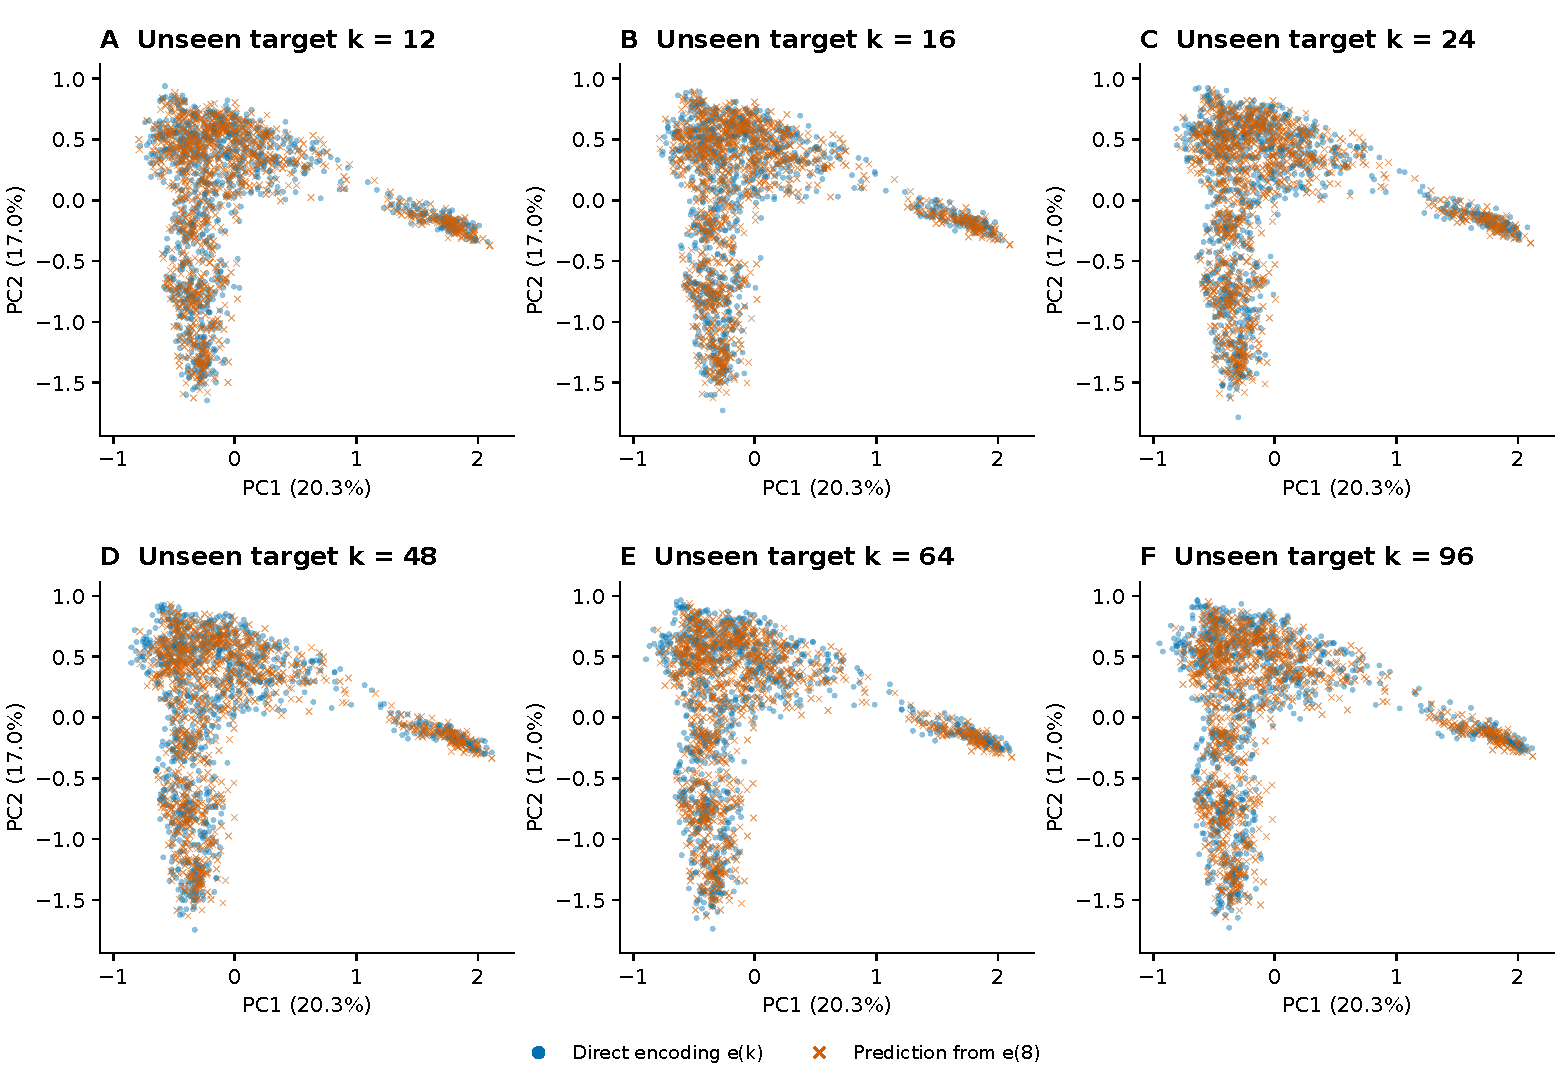
\includegraphics[width=\linewidth]{figures/case_all_unseen_pca_no_pair_lines.pdf}
\caption{\textbf{All six unseen target states in the E16.5 E1S1 case.} Every panel uses the same PCA basis and the same 1,024 positions. Metrics are computed in 256 dimensions. Targets and predictions are paired at each location.}
\label{fig:ode-case-all-pca}
\end{figure}
\begin{table}[!htbp]
\centering\small
\caption{\textbf{Full-dimensional accuracy underlying the case PCA.} MSE ratio compares prediction with unchanged $e_8$ against directly encoded targets; NRMSE and $R^2$ use the same full-dimensional targets.}
\label{tab:ode-case-pca}
\begin{tabular}{lccc}
\toprule
Target $k$ & MSE ratio & NRMSE & $R^2$ \\
\midrule
12 & 0.884 & 0.206 & 0.958 \\
16 & 0.810 & 0.243 & 0.941 \\
24 & 0.739 & 0.280 & 0.922 \\
48 & 0.664 & 0.333 & 0.889 \\
64 & 0.643 & 0.352 & 0.876 \\
96 & 0.621 & 0.377 & 0.858 \\
\bottomrule
\end{tabular}

\end{table}

\FloatBarrier
\subsection{Context-response evaluation across observation ranges}
\label{app:response-meaning}

\paragraph{Matched response definitions and sampling.}
For $\widehat e_i(k)=T_{8\to k}(e_{i,8})$, Figure~\ref{fig:granularity-query-summary}c, Figure~\ref{fig:ode-context}a and the grouping in Figure~\ref{fig:facial-nerve-composition} use
\[
D_i^{\mathrm{pred}}(a,b)=
\frac{\|\widehat e_i(b)-\widehat e_i(a)\|_2}{\sqrt d\,\log_2(b/a)},\qquad
D_i^{\mathrm{enc}}(a,b)=
\frac{\|e_i(b)-e_i(a)\|_2}{\sqrt d\,\log_2(b/a)}.
\]
Both operands in the predicted displacement belong to queries from the same fixed $e_8$. Encoded states are evaluation references, and all displayed doubling intervals have log width one.

Held-out comparisons use 1,024 fixed locations per section. Anatomical cases use the training sections identified in Table~\ref{tab:evaluation_protocol}, with up to 128 locations per annotation selected by a fixed hash of observation identity; smaller domains retain every location.

\paragraph{Held-out location ordering.}
For each held-out section and each doubling interval, we sort the 1,024 locations by predicted response and split them into four equal groups; ties preserve sample order. We compare the directly encoded changes in the lowest and highest quarters. Figure~\ref{fig:granularity-query-summary}c averages these group means over the four intervals within each section, giving eight paired section means.

\paragraph{Actual neighborhood composition.}
Let $q_{ic}(k)$ be the proportion of annotation $c$ among the $k-1$ neighbors after excluding the focal center. For the same interval as the response,
\[
C_i(a,b)=\tfrac12\sum_c|q_{ic}(b)-q_{ic}(a)|.
\]
Support ordering is identical to the model input, and unknown-label mass is retained. The Facial nerve composition bars (Figure~\ref{fig:facial-nerve-composition}) follow the same 16 locations in each extreme predicted-response quarter. Their mean encoded changes are 0.0191 and 0.0343 in the low and high groups, respectively (ratio 1.799). Corresponding mean TV values are 0.134 and 0.284. Composition TV quantifies the change in annotated tissue proportions.

\begin{figure}[!htbp]
\centering
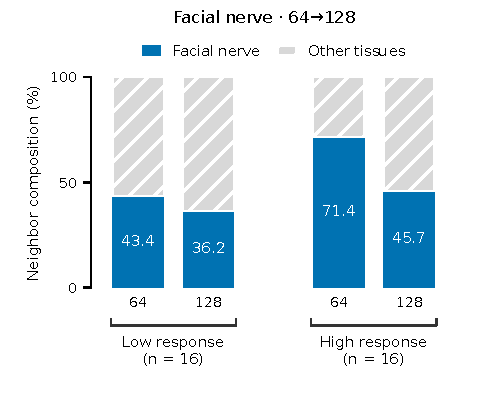
\includegraphics[width=0.58\linewidth]{figures/facial_nerve_composition.pdf}
\caption{\textbf{Neighborhood composition in low- and high-response Facial nerve locations.} The groups are the lowest and highest predicted-response quarters among all 64 Facial nerve locations in the E14.5 E1S1 training section, using the $64\to128$ response in Figure~\ref{fig:ode-context}a. Each pair of bars follows the same 16 locations at both granularities. Blue shows the mean Facial nerve fraction; gray shows all other labels. Predictions start from fixed $e_8$.}
\label{fig:facial-nerve-composition}
\end{figure}

\paragraph{Within-Brain changes under a constant annotation.}
Among sampled Brain locations whose neighborhoods remain entirely Brain-labeled at both $r=8$ and $r=16$, predicted responses correlate with directly encoded changes (Spearman $\rho=0.645$), showing molecular-context variation within a constant anatomical annotation.

\paragraph{Whole-section spatial overview.}
Figure~\ref{fig:ode-context}b averages the instantaneous response $s_i(2^t)=\|f_\theta(z_i((t-3)/4),(t-3)/4)\|_2/(4\sqrt d)$ over 64 equally spaced midpoints in $t=\log_2 k\in[3,7]$. This path average differs from the finite response used in panel (a) and to define the groups in Figure~\ref{fig:facial-nerve-composition}. Colors use an empirical percentile reference pooled over the full-range mean and the four doubling-range means, with all 121,767 locations included. Panel (c) shows observed composition TV from 8 to 128. The maps show spatial distributions without smoothing; their whole-section Spearman correlation is 0.174. Both maps are rotated together by $180^\circ$ relative to the source coordinates for display, preserving distances and the common orientation. Spatial scale bars use the nominal $25\,\mu$m pitch of the bin50 matrices~\citep{chen2022mosta}; response remains normalized by $\log_2 k$.
